\documentclass[14pt, a4paper]{report}
\usepackage{mathtext}
\usepackage[T2A]{fontenc}
\usepackage[utf8]{inputenc}
\usepackage[russian]{babel}
\usepackage{multirow}
\usepackage{slashbox}
\usepackage{makecell}
\usepackage{graphicx}
\usepackage{physics}
\usepackage{amstext}
\usepackage{caption}
\usepackage{subcaption}
\usepackage{cmap}
\usepackage{float}

\renewcommand{\thesection}{\arabic{section}.}
\renewcommand{\thesubsection}{\arabic{section}.\arabic{subsection}.}

\title{\textbf{Отчет о выполнении лабораторной работы 4.7.2 "Эффект Покельса"}}
\author{Алпатова Александра, Калашников Михаил, Б03-205}
\date{}

\begin{document}
\maketitle

\textbf{Цель работы:}
исследовать интерференцию рассеянного света, прошедшего кристалл; наблюдать изменение характера поляризации света при наложении на кристалл электрического поля.
\newline

\textbf{В работе используются:}
\begin{itemize}
\item гелий-неоновый лазер;
\item поляризатор;
\item кристалл ниобата лития ($n_0=2.29, l=26\ мм$);
\item матовая пластинка;
\item экран;
\item источник высоковольтного переменного и постоянного напряжения;
\item фотодиод;
\item осциллограф;
\item линейка.
\end{itemize}

\section{Теоретические сведения}

\section{Экспериментальная установка}

\section{Проведение эксперимента и обработка данных}

\begin{enumerate}

\setcounter{enumi}{0}

\item Соберем оптическую схему. С помощью поляризатора убедимся, что лазерный луч поляризован вертикально.

\item Поставим кристалл и установим матовую пластину. Система распологается на расстоянии $L=80\ см$ от экрана.

\item Получим на экране интерференционную картину. Добьемся совмещения центра коноскопической картины с положением луча на экране в отсутствии матовой пластинки.

\item Проведем измерения темных колец $r(m)$. Построим график $r^2=f(m)$. 
\begin{figure}[H]
\centering
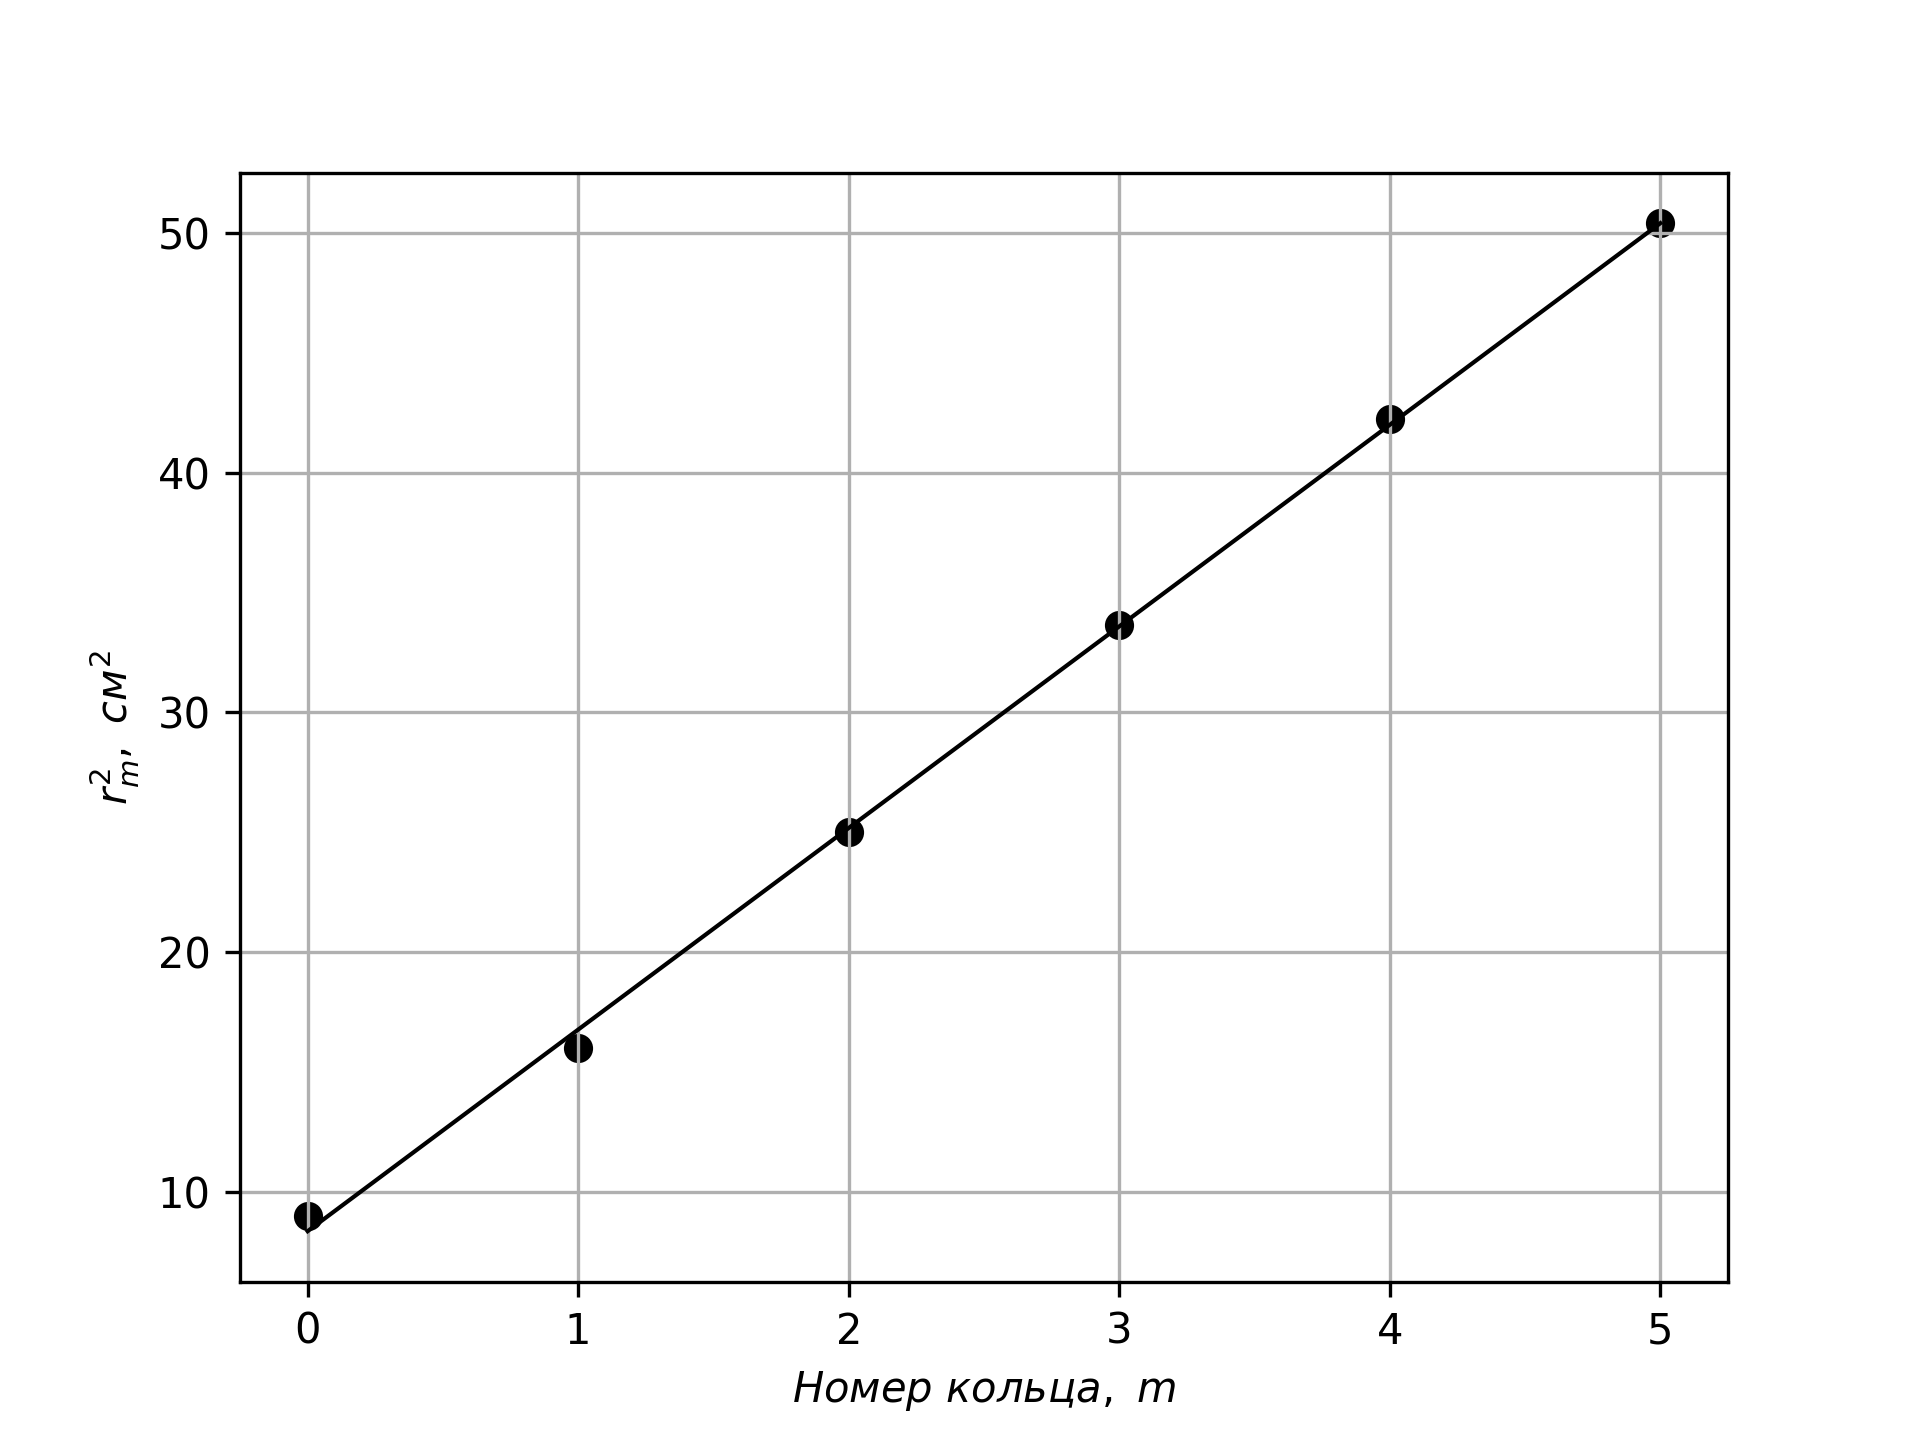
\includegraphics[scale=0.6]{images/472_2.png}
\caption{График зависимости $r^2=f(m)$}
\end{figure}

По углу наклона прямой и с помощью формулы
\[r^2=\frac{\lambda}{l}\frac{(n_0L)^2}{n_0-n_e}\]
определим двулучевое преломление: $(n_0-n_e)=8.1\cdot10^{-5}$

\item Подключим разъем блока питания на постоянное напряжение и включим блок питания в сеть. При повышении напряжения яркость пятна на экране сначала увеличивается и достигает максимума при $U=U_{\lambda/2}=30\ дел$. Затем яркость снижается и достигаем минимума при $U=U_{\lambda}=60\ дел$. Проделаем то же самое для параллельных поляризаций и получим, что $U=U_{\lambda/2}=31\ дел$, $U=U_{\lambda/2}=62\ дел$.

\end{enumerate}

\section{Приложения}

\begin{figure}[H]
\centering
\includegraphics[scale=0.15]{images/472_1.png}
\caption{Полученная картина}
\end{figure}

\begin{figure}[H]
\centering
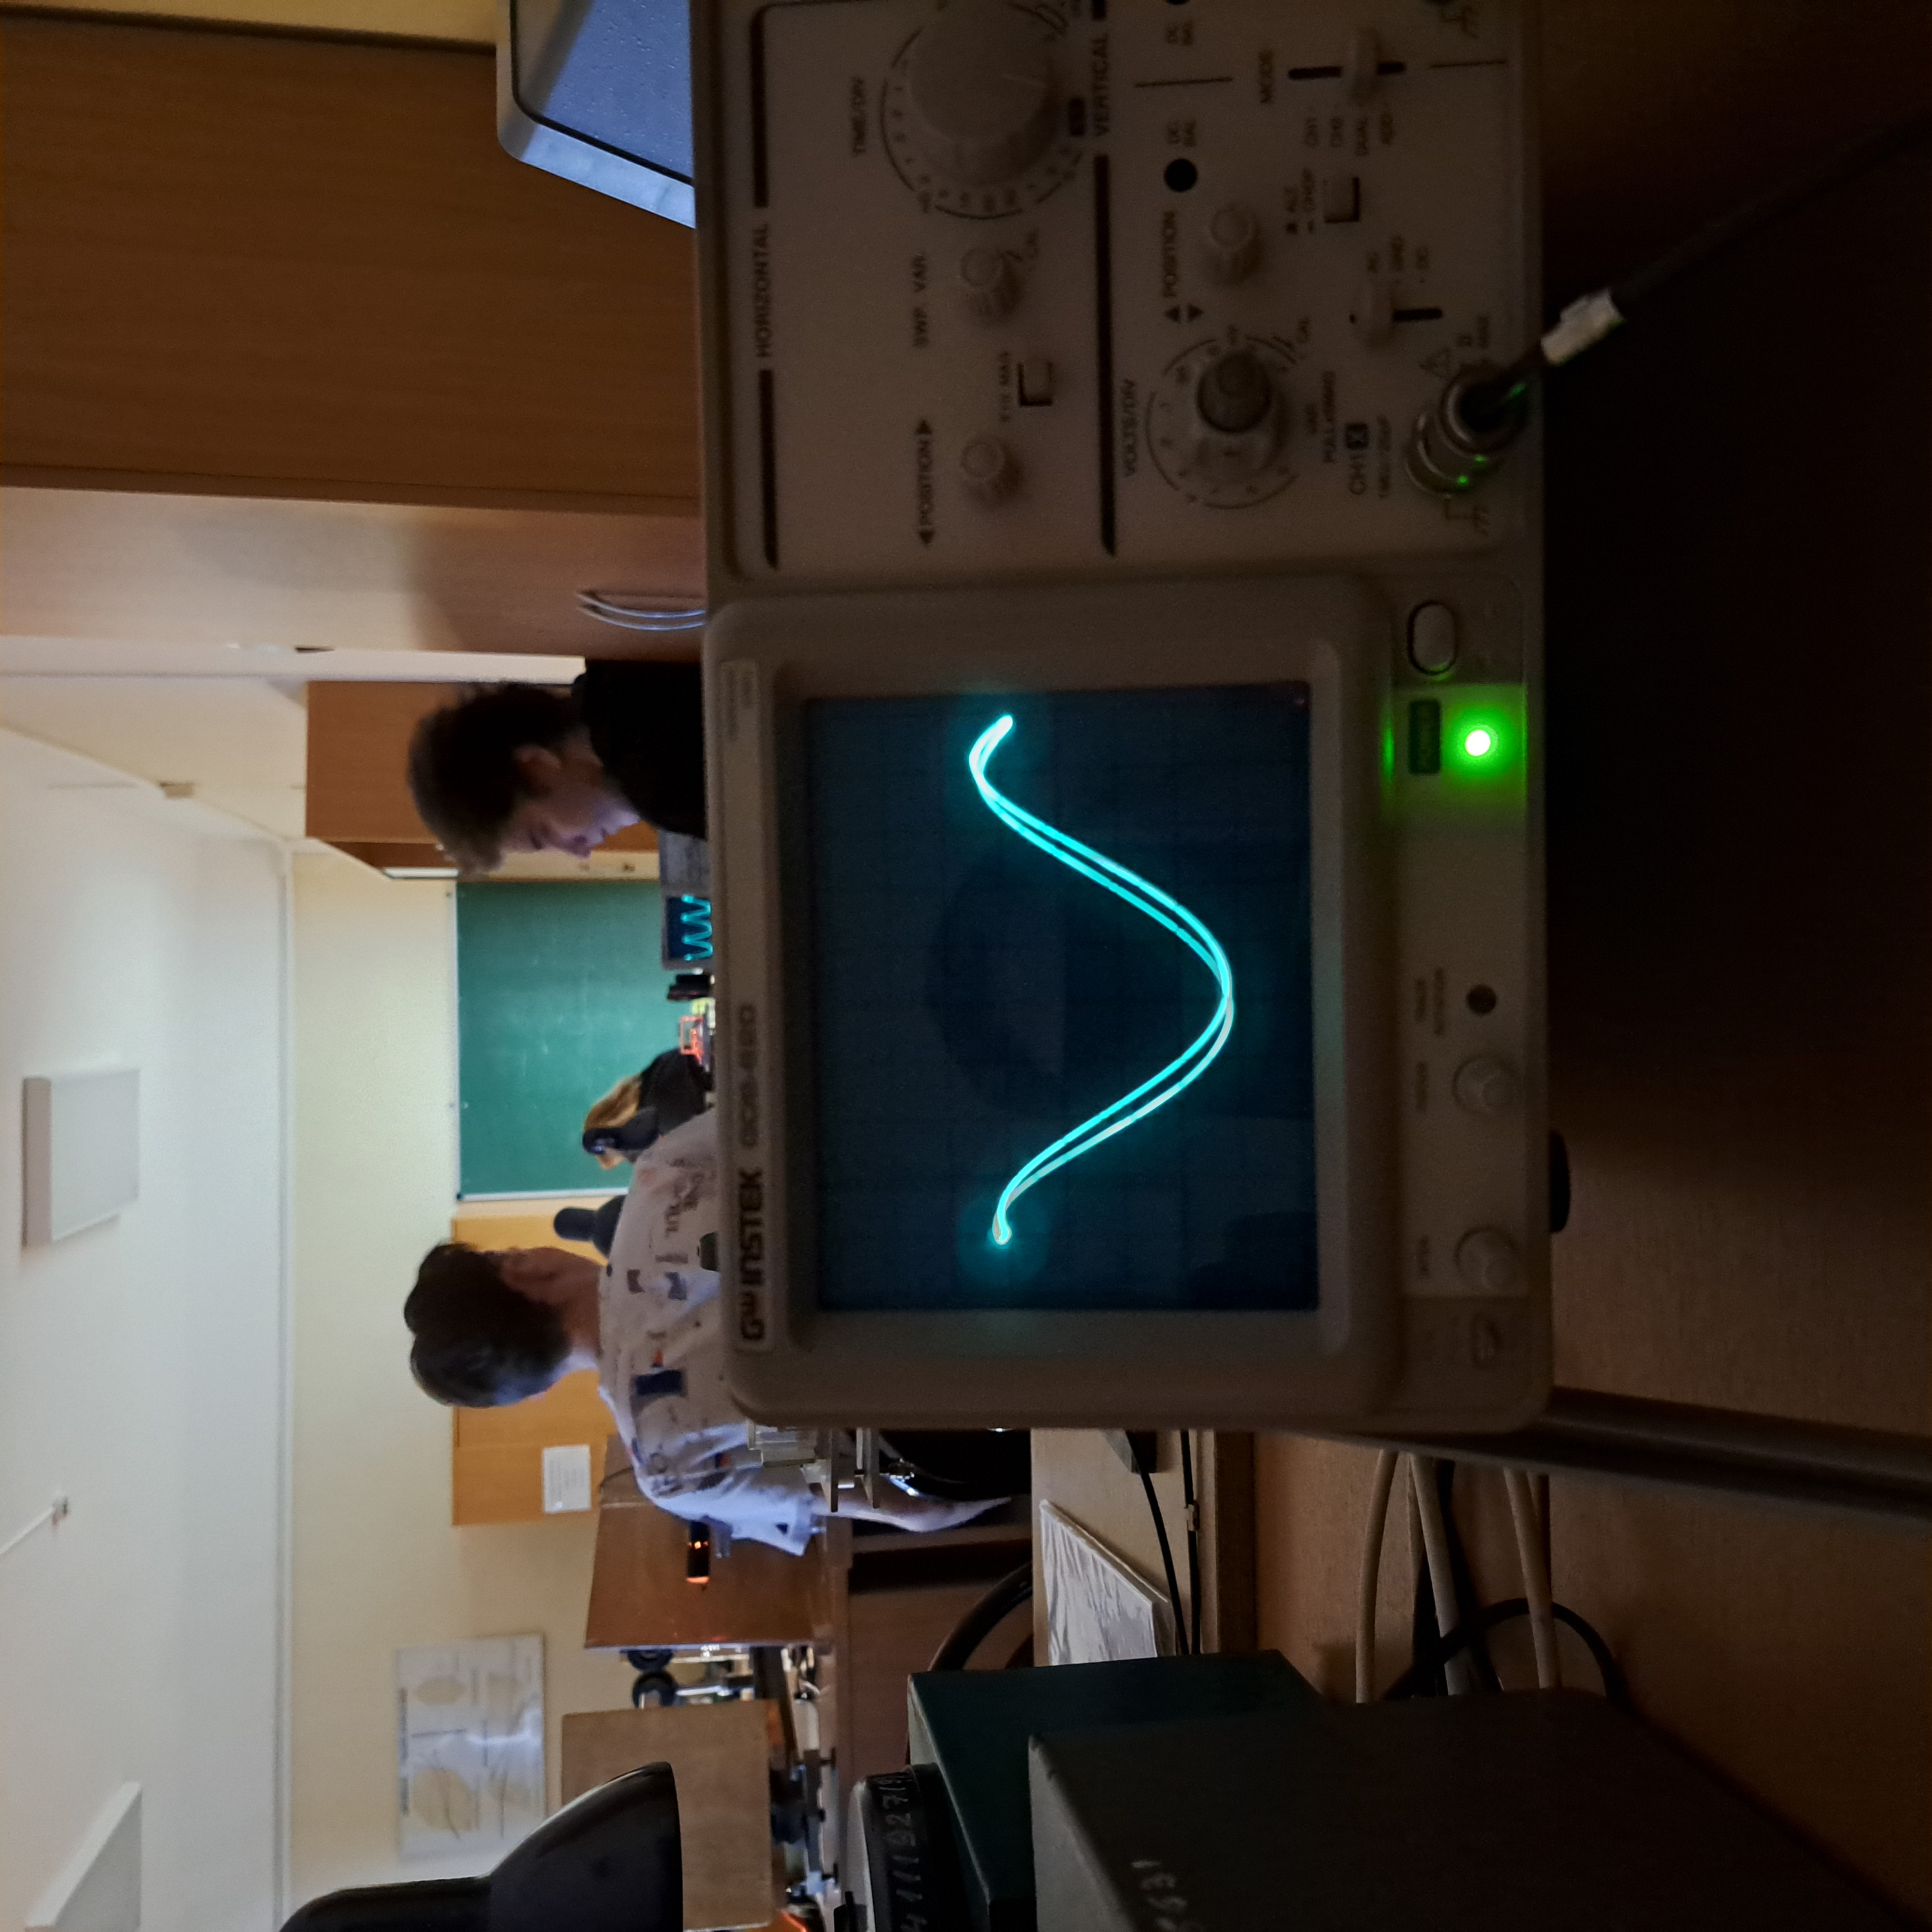
\includegraphics[scale=0.1]{images/472_3.jpg}
\end{figure}

\begin{figure}[H]
\centering
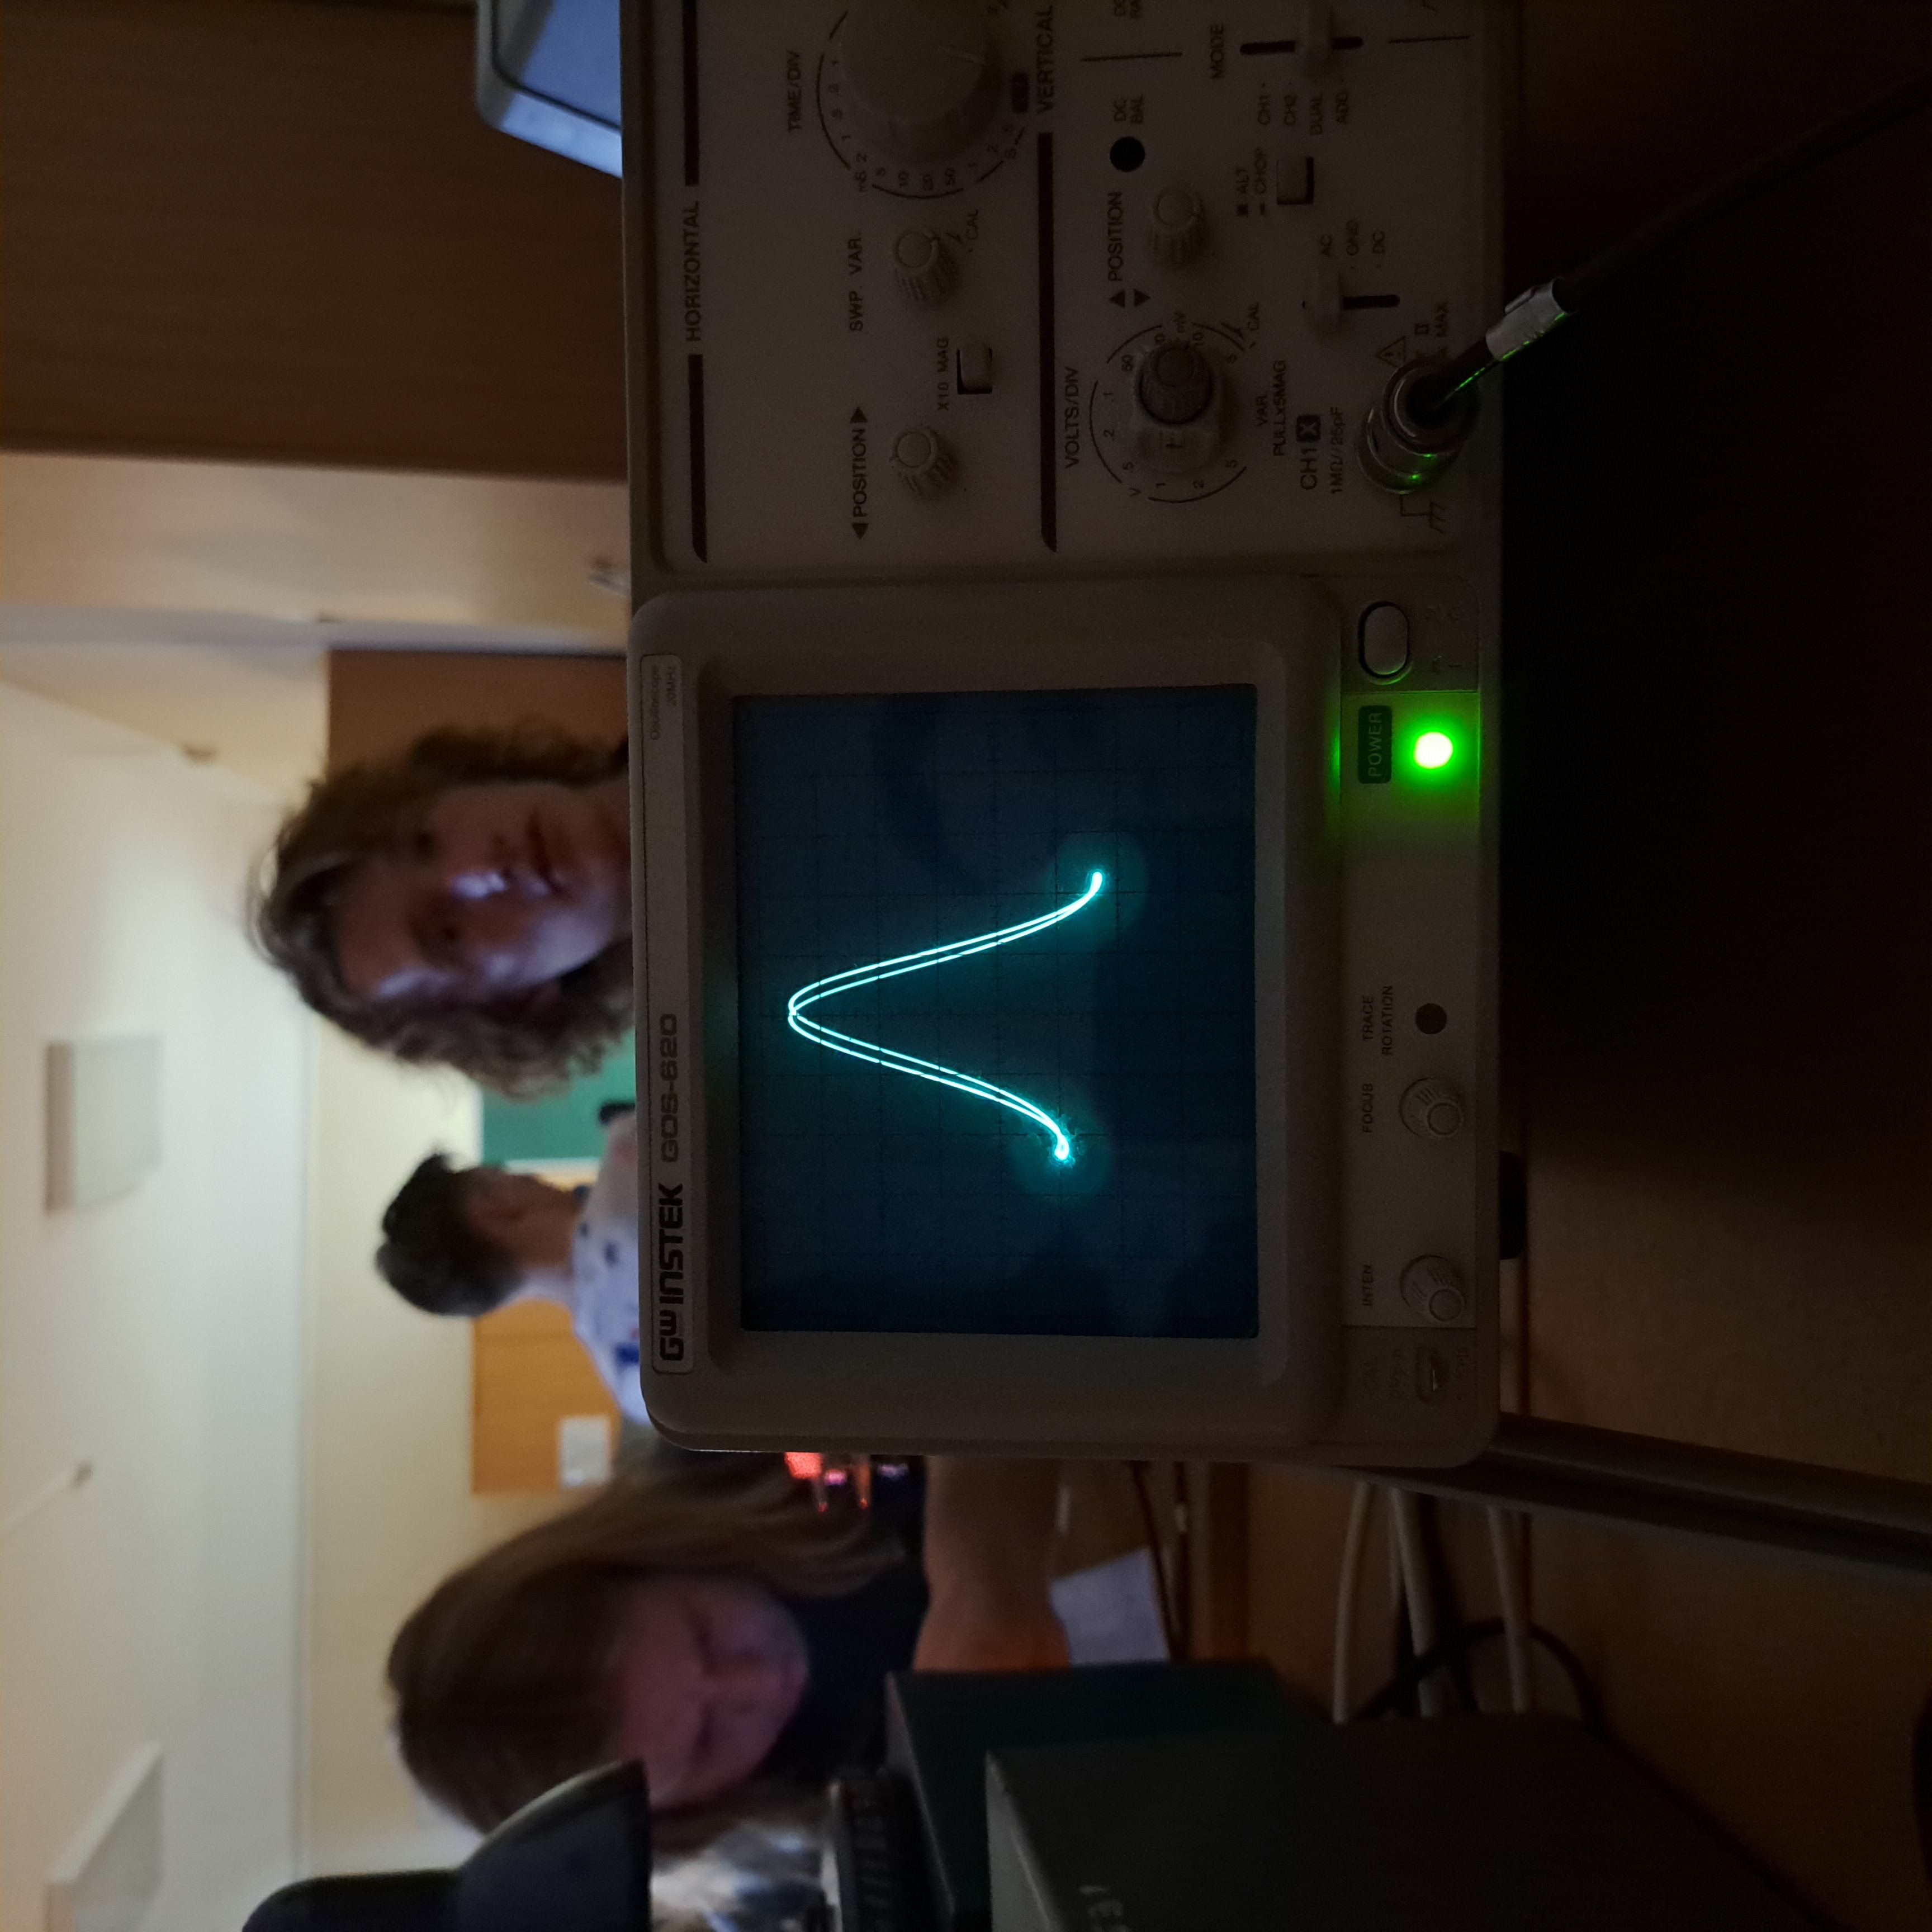
\includegraphics[scale=0.1]{images/472_4.jpg}
\end{figure}


\end{document}